In order to train a complex network like LSTMs, a large data set is required. Ideally, the data would have low missingness, as missing values can impact training effectiveness (this is true for all networks, although the issue becomes more pronounced when data are time-dependent). Additionally, the data should not have any seasonal increase over time. Due to these requirements, the training data were selected to be water depth time series collected within the Everglades National Park (EVER). There are 52 monitoring stations present, all with various levels of missingness. The chosen station, P33, had less than 1\% missingness and had only a minor increasing trend (see Figure \ref{fig:P33}).

\begin{figure}[ht]
    \centering
    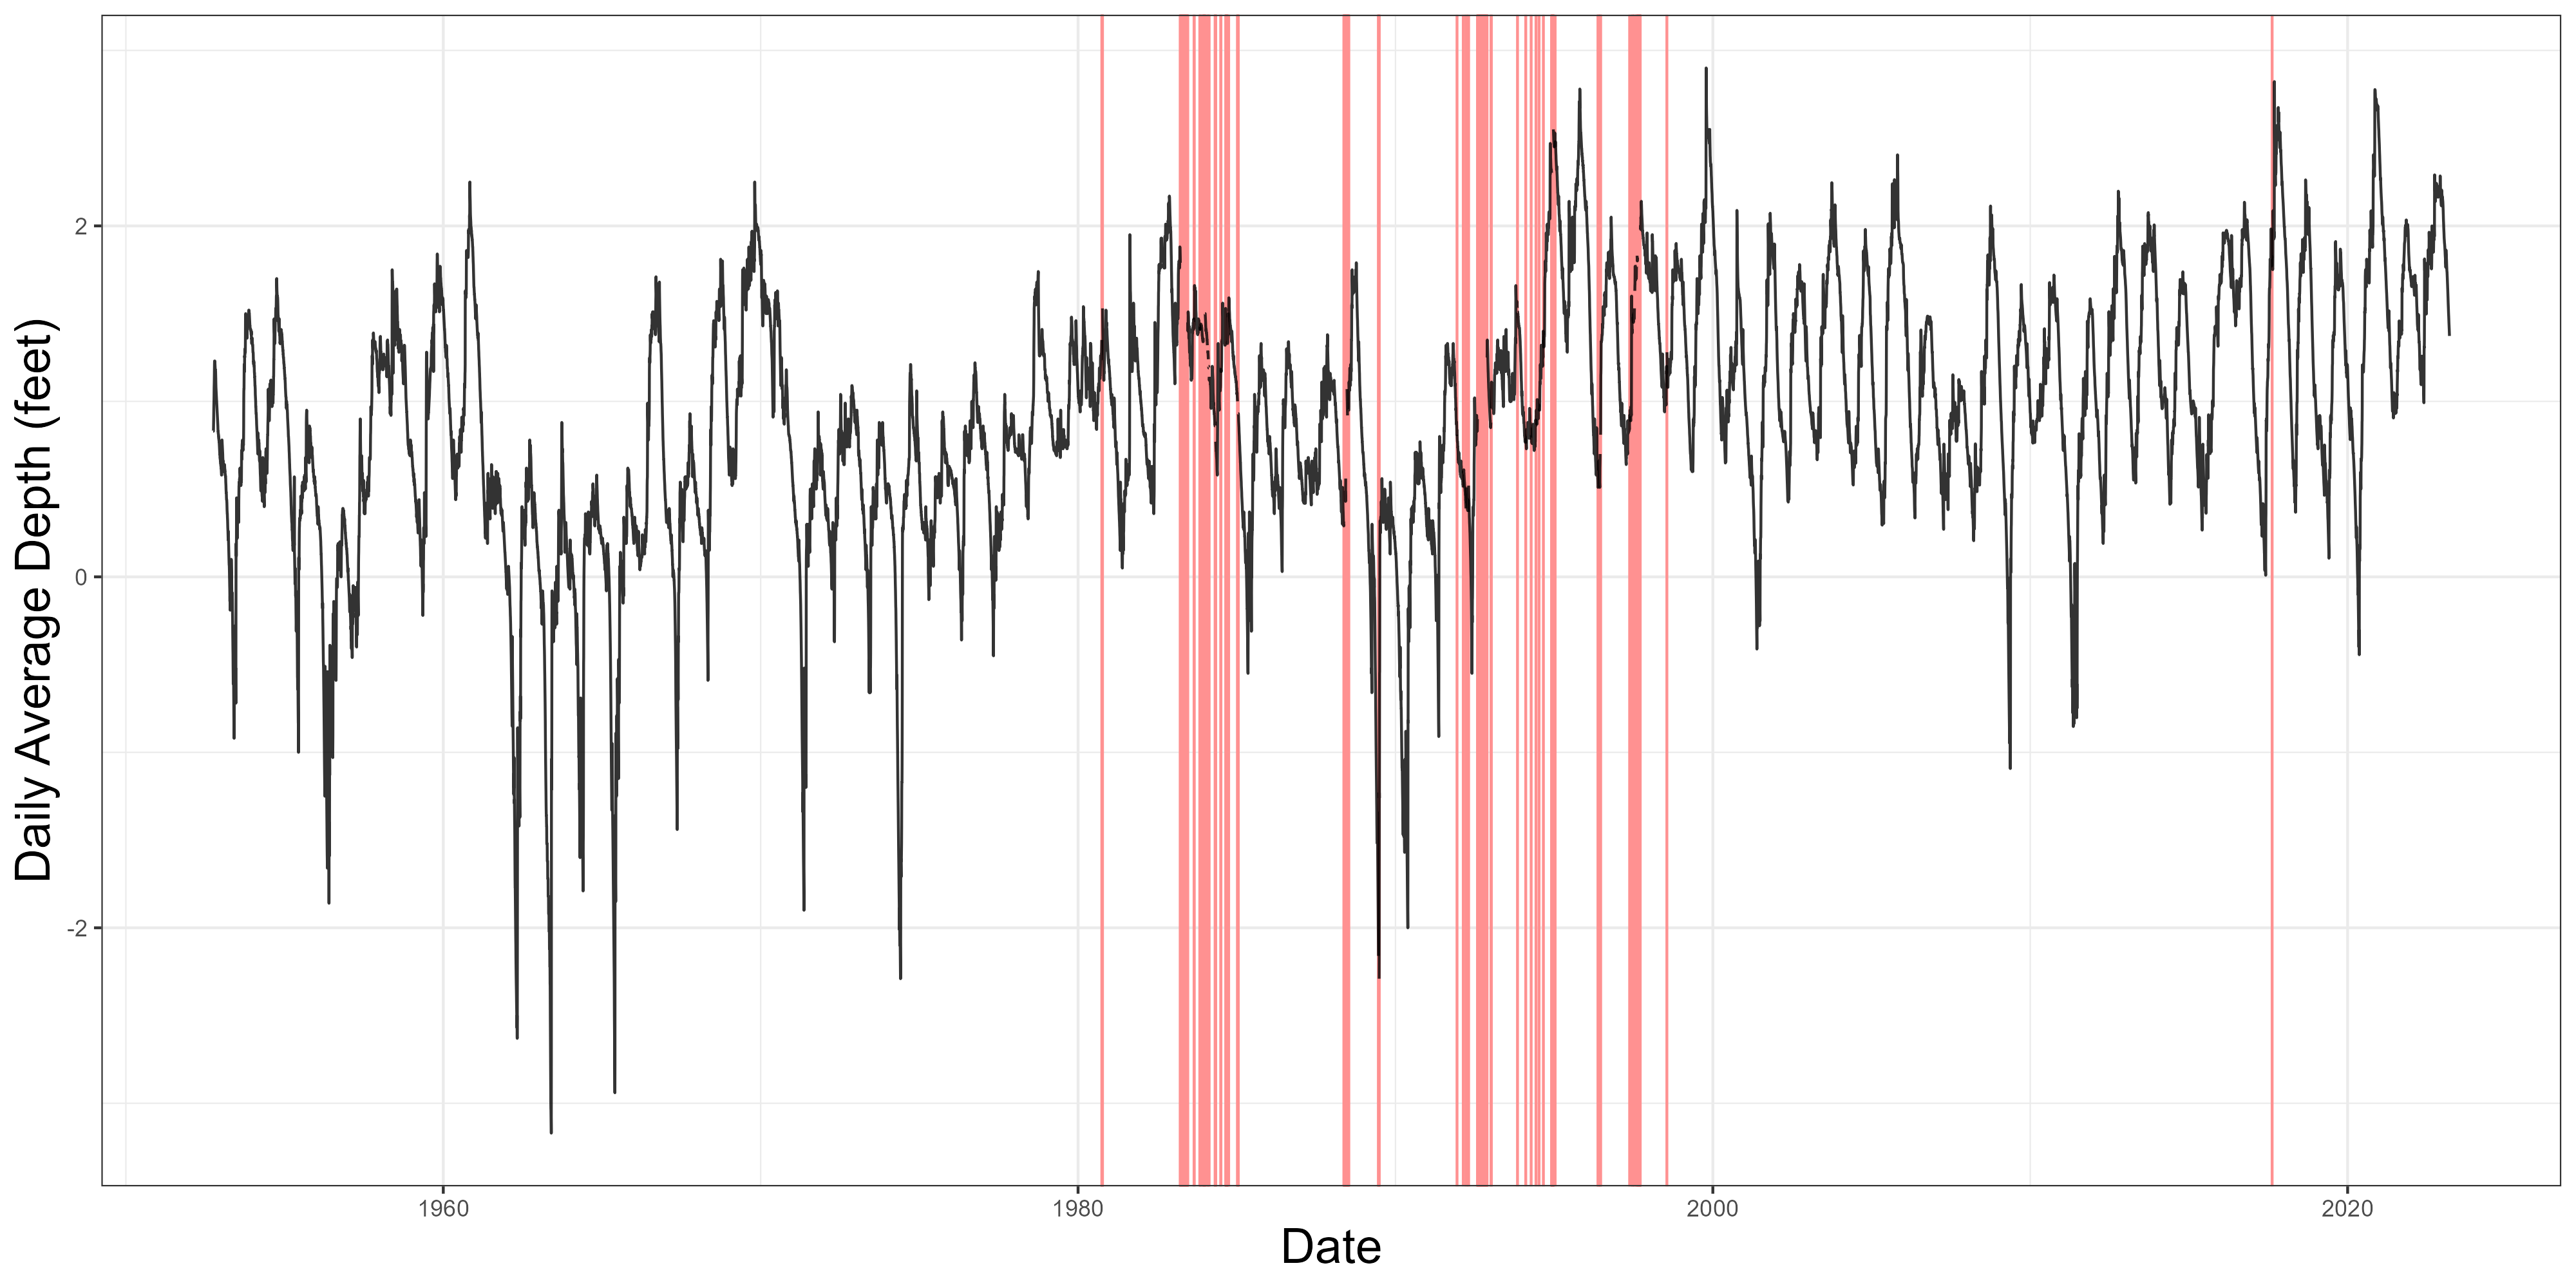
\includegraphics[width=0.9\linewidth]{"Figures/P33_Time_Series_Missingness.png"}
    \caption{A line plot of the time series used to train the LSTM in this project. Red vertical bars indicate a date with a missing value.}
    \label{fig:P33}
\end{figure}

Due to the present although low missingness, an interpolation method had to be chosen to impute those missing values. Several candidate algorithms were tested, but eventually the decision to use a Kalman filter was made \citep{kalmanfilter}. The line plot in Figure \ref{fig:P33_Interpolated} displays the imputed values for the date range of 1960 to 2000.

\begin{figure}[ht]
    \centering
    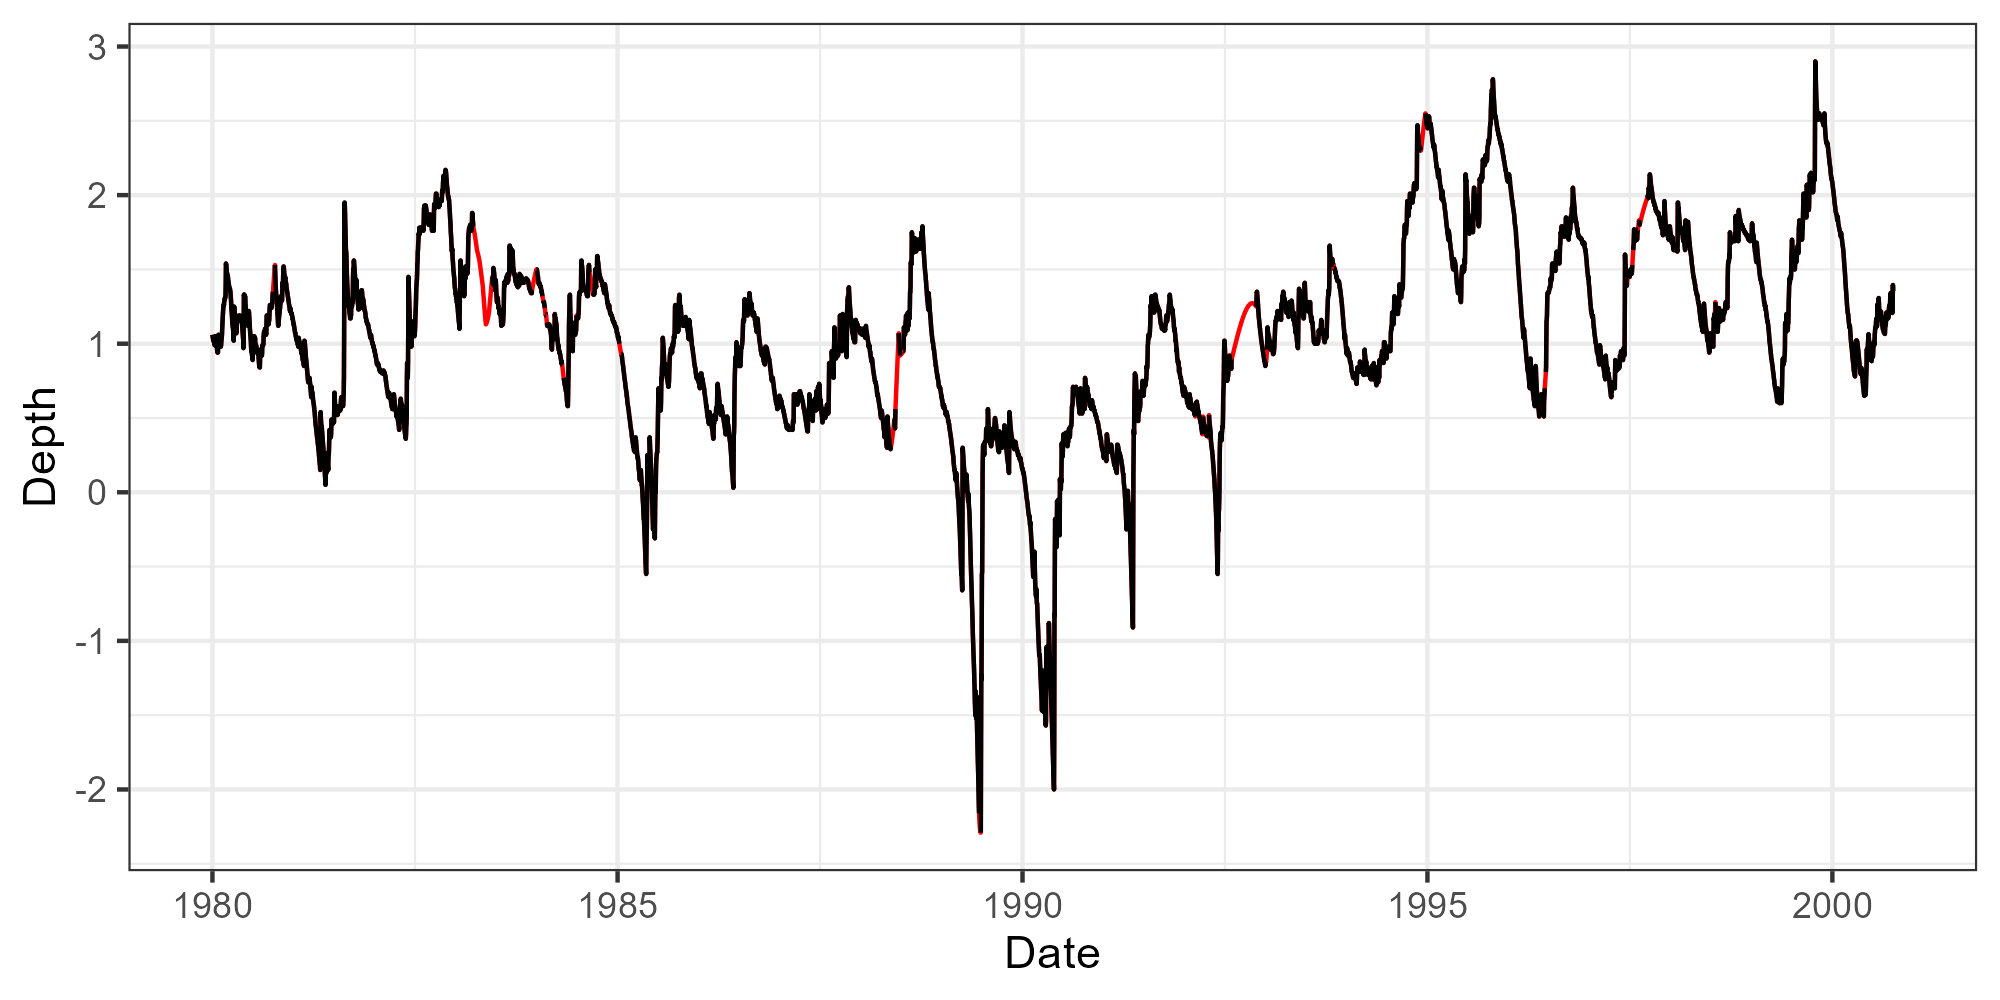
\includegraphics[width=0.9\linewidth]{"Figures/Interpolation_60_20.png"}
    \caption{A line plot of the time series used to train the LSTM in this project. Red lines indicate the imputed values using the Kalman filter. Note that this plot focuses on 1980 to 2000, despite imputation being performed across the entire time series.}
    \label{fig:P33_Interpolated}
\end{figure}